\documentclass[11pt, a4paper]{article}

% Volle Seite nutzen
\usepackage{fullpage} 
\headsep 1cm
\parindent 0cm

\usepackage[utf8]{inputenc}
\usepackage{minted}
\usepackage{graphicx}
\usepackage{caption}
\usepackage{makecell}
\usepackage{subcaption}
\usepackage{hyperref}
\usepackage{amsmath}
\usepackage{float}

\title{Benchmark of two PHP GraphQL implementations }
\author{joon}
\date{June 2021}

\begin{document}

\maketitle

\section{Introduction}
This document should give an impression of the speed of the new PHP GraphQL implementation \textbf{\hyperlink{https://github.com/joonlabs/php-graphql}{joonlabs/php-graphql}}. A comparison to the currently most popular PHP GraphQL implementation \textbf{\hyperlink{https://github.com/webonyx/graphql-php}{webonyx/graphql-php}} is drawn. Both libraries are tested with the same schema and the same queries on to different server setups each, to allow a consistent but also real-use-case like comparison. The schema that is used, is the Star Wars schema, which is included in both libraries.

\section{Setup and Reproduction}
This benchmark is performed using curl. After both implementations are started on one server each, a shell script executes a specified query 200 times against each of these two servers. In order to avoid influences by cold restarts, each query is executed 5 times before starting to record the data. A random comment is added to each query every call to prevent server-side caching. The response time of each curl request is stored and once all queries finished, they are combined into a JSON file.  The resulting JSON file is then analyzed and values such as the mean and standard deviation are calculated.

This benchmark uses four different queries, which represent different levels of complexity, to evaluate the parsing, validation and execution of both implementations. The four queries can be found in the appendix, as can the measurement results. 

To make this comparison as reproducible as possible, a separate Git repository is available at \url{https://github.com/joonlabs/graphql-benchmarks}, which contains the benchmark scripts and both schema implementations.

The benchmarks for this document were run on a local PHP built-in server on a MacBook Pro (13'', M1, 2020) with PHP v7.4.1 and on an Apache web server in production mode at \hyperlink{https://graphql.joonlabs.com/}{https://graphql.joonlabs.com/} running PHP v7.3.25. Multithreading was not enabled in either server.


\section{Results}
For performance differences in percent, the following formular is used, where $t_{faster}$ is the response time of the faster server and $t_{slower}$ is the response time of the slower server:
\begin{align}
    \Delta p = 1 - \frac{t_{faster}}{t_{slower}}
\end{align}
Looking at table \ref{table_1} we can see that \textbf{joonlabs/php-graphql} outperforms \textbf{webonyx/graphql-php} by 52.42\%, running the query Q1. Running the query Q2,  \textbf{joonlabs/php-graphql} is 17.84\% faster and running the query Q4, it is 3.84\% faster. When running the Query Q3, both libraries seem to perform equally while \textbf{webonyx/graphql-php} is (on average) 1.1ms faster regarding this query. Because these benchmarks were run on a local server the standard deviation is low, as there have not been any external network influences like packet loss, connection issues, etc. For a detailed look at the data, take a look at table \ref{table_1} and the figure \ref{figure1}.

In comparison to that, when looking at table \ref{table_2} (and figure \ref{figure2}) we can now see the network influence, represented by the higher standard deviation. Here a standard deviation of about 13ms to 80ms is always present. Despite that, you can still see the speed differences between the two libraries, as \textbf{joonlabs/php-graphql} outperforms \textbf{webonyx/graphql-php} here as well. A total difference in the measured response time of 5ms to 20ms can be obtained for each query in average.

\section{Discussion}
As described above, we can obtain that \textbf{joonlabs/php-graphql} outperforms \textbf{webonyx/graphql-php} in terms of speed in the most example queries of this benchmark. Despite this fact it must be said, that this document is not meant to be evidence or a statement that one of the libraries is better than the other. Both libraries follow different approaches and have different strengths and weaknesses. This document should only provide a reproducible possibility to enable an independent benchmark with as real-world influences as possible and to compare response times. Also only the Star Wars schema is tested here, which should not be used solely as a basis for an absolute speed evaluation or comparison, since schemas in real-world use cases usually deviate strongly from one another in size, complexity and area of application.

\clearpage
\section{Appendix}


\begin{table}[H]
\centering
\begin{tabular}{ |c||c||c|c||c|c|  }
 \hline
Query & Iterations & \makecell{\textbf{joonlabs}\\mean (ms)} & \makecell{\textbf{webonyx}\\mean (ms)} & \makecell{\textbf{joonlabs}\\SD (ms)} & \makecell{\textbf{webonyx}\\SD (ms)} \\
 \hline
 Q1 & 200 & \textbf{12.59} & 26.46 & 0.34 & 0.32\\
 Q2 & 200 & \textbf{29.11} & 35.43 & 0.35 & 0.32\\
 Q3 & 200 & 1099.11 & \textbf{1097.95} & 4.77 & 5.39\\
 Q4 & 200 & \textbf{46.13} & 47.97 & 0.48 & 0.32\\
 \hline
\end{tabular}
\caption{Test results, running on the local PHP built-in server}
\label{table_1}
\end{table}


\begin{table}[H]
\centering
\begin{tabular}{ |c||c||c|c||c|c|  }
 \hline
Query & Iterations & \makecell{\textbf{joonlabs}\\mean (ms)} & \makecell{\textbf{webonyx}\\mean (ms)} & \makecell{\textbf{joonlabs}\\SD (ms)} & \makecell{\textbf{webonyx}\\SD (ms)} \\
 \hline
 Q1 & 200 & \textbf{139.80} & 162.43 & 13.32 & 76.06\\
 Q2 & 200 & \textbf{148.33} & 167.68 & 13.00 & 78.18\\
 Q3 & 200 & \textbf{164.24} & 169.01 & 74.89 & 17.91\\
 Q4 & 200 & \textbf{185.55} & 195.30 & 76.53 & 79.08\\
 \hline
\end{tabular}
\caption{Test results run on an Apache web server}
\label{table_2}
\end{table}

\clearpage

\textbf{Query 1 - referenced as Q1}
\begin{minted}{gql.py:GraphqlLexer -x}
{
  hero{
    name
  }
}
\end{minted}

\textbf{\\Query 2 - referenced as Q2}
\begin{minted}{gql.py:GraphqlLexer -x}
query{
  hero(episode: JEDI){
    id
    name
    appearsIn
    secretBackstory
    friends{
      id
      name
      ... on Droid{
        appearsIn
        primaryFunction
      }
      ... on Human{
        appearsIn
        secretBackstory
      }
      ... HumanFragment
    }
  }
}

fragment HumanFragment on Human{
	id
    name
    appearsIn
    secretBackstory
    friends{
      id
      name
      ... on Droid{
        appearsIn
        primaryFunction
      }
      ... on Human{
        appearsIn
        secretBackstory
      }
    }
}
\end{minted}

\textbf{\\Query 3 - referenced as Q3}
\begin{minted}{gql.py:GraphqlLexer -x}
query{
  human(id:"1001"){
    ... HumanFragment
  }
  droid(id:"2001"){
    ... DroidFragment
  }
  hero(episode: JEDI){
    id
    name
    appearsIn
    secretBackstory
    friends{
      id
      name
      ... on Droid{
        appearsIn
        primaryFunction
      }
      ... on Human{
        appearsIn
        secretBackstory
      }
      ... HumanFragment
    }
  }
}

fragment HumanFragment on Human{
	id
    name
    appearsIn
    secretBackstory
    friends{
      id
      name
      ... on Droid{
        appearsIn
        primaryFunction
        friends{
          ... CharacterFragment
        }
      }
      ... on Human{
        appearsIn
        secretBackstory
        friends{
          ... CharacterFragment
        }
      }
    }
}

fragment DroidFragment on Droid{
	id
    name
    appearsIn
    primaryFunction
    friends{
      id
      name
      ... on Droid{
        appearsIn
        primaryFunction
        friends{
          ... CharacterFragment
        }
      }
      ... on Human{
        appearsIn
        secretBackstory
        friends{
          ... CharacterFragment
        }
      }
    }
}

fragment CharacterFragment on Character{
  id
  name
  friends{
    name
  }
}
\end{minted}

\textbf{\\Query 4 - referenced as Q4}
\begin{minted}{gql.py:GraphqlLexer -x}
IntrospectionQuery {
    __schema {
      queryType { name }
      mutationType { name }
      subscriptionType { name }
      types {
        ...FullType
      }
      directives {
        name
        description
        args {
          ...InputValue
        }
      }
    }
  }

  fragment FullType on __Type {
    kind
    name
    description
    fields(includeDeprecated: true) {
      name
      description
      args {
        ...InputValue
      }
      type {
        ...TypeRef
      }
      isDeprecated
      deprecationReason
    }
    inputFields {
      ...InputValue
    }
    interfaces {
      ...TypeRef
    }
    enumValues(includeDeprecated: true) {
      name
      description
      isDeprecated
      deprecationReason
    }
    possibleTypes {
      ...TypeRef
    }
  }

  fragment InputValue on __InputValue {
    name
    description
    type { ...TypeRef }
    defaultValue
  }

  fragment TypeRef on __Type {
    kind
    name
    ofType {
      kind
      name
      ofType {
        kind
        name
        ofType {
          kind
          name
        }
      }
    }
  }
\end{minted}

\clearpage
\begin{figure}
\centering
\begin{subfigure}{.5\textwidth}
  \centering
  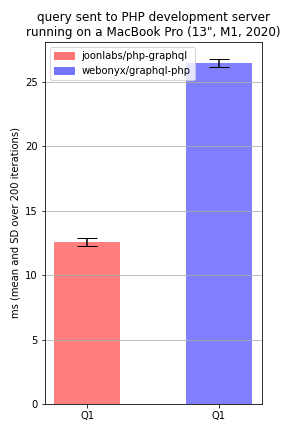
\includegraphics[width=.75\linewidth]{results/localhost_Q1.png}
  \label{localhost_Q1}
\end{subfigure}%
\begin{subfigure}{.5\textwidth}
  \centering
  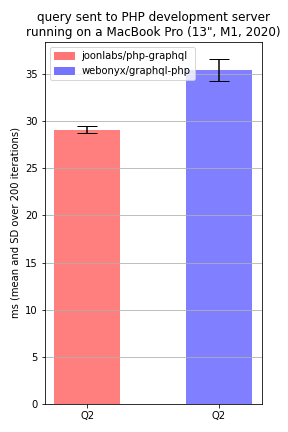
\includegraphics[width=.75\linewidth]{results/localhost_Q2.png}
  \label{localhost_Q2}
\end{subfigure}%
\\
\begin{subfigure}{.5\textwidth}
  \centering
  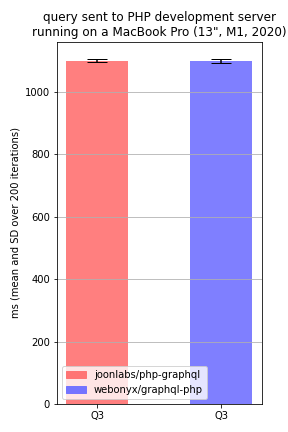
\includegraphics[width=.75\linewidth]{results/localhost_Q3.png}
  \label{localhost_Q3}
\end{subfigure}%
\begin{subfigure}{.5\textwidth}
  \centering
  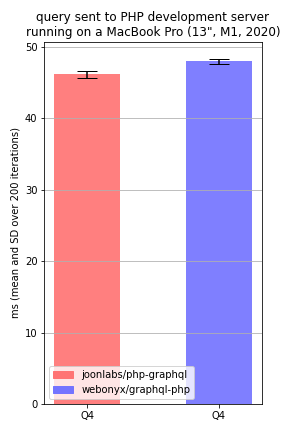
\includegraphics[width=.75\linewidth]{results/localhost_Q4.png}
  \label{localhost_Q4}
\end{subfigure}%
\caption{Test results, running on the local PHP built-in server}
\label{figure1}
\end{figure}


\begin{figure}
\centering
\begin{subfigure}{.5\textwidth}
  \centering
  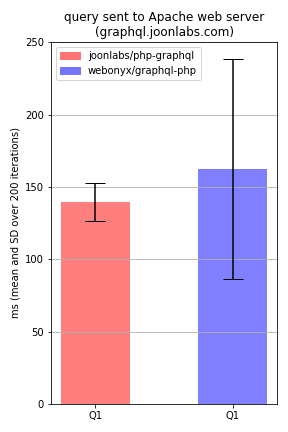
\includegraphics[width=.75\linewidth]{results/joonlabs_Q1.png}
  \label{localhost_Q1}
\end{subfigure}%
\begin{subfigure}{.5\textwidth}
  \centering
  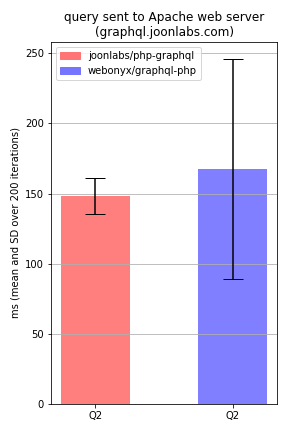
\includegraphics[width=.75\linewidth]{results/joonlabs_Q2.png}
  \label{localhost_Q2}
\end{subfigure}%
\\
\begin{subfigure}{.5\textwidth}
  \centering
  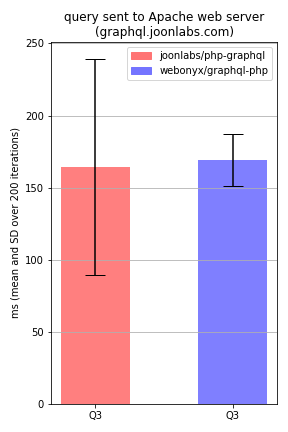
\includegraphics[width=.75\linewidth]{results/joonlabs_Q3.png}
  \label{localhost_Q3}
\end{subfigure}%
\begin{subfigure}{.5\textwidth}
  \centering
  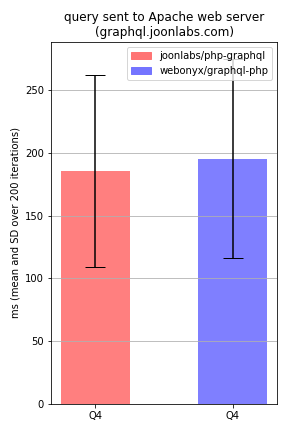
\includegraphics[width=.75\linewidth]{results/joonlabs_Q4.png}
  \label{localhost_Q4}
\end{subfigure}%
\caption{Test results run on an Apache web server at https://graphql.joonlabs.com}
\label{figure2}
\end{figure}

\end{document}
